\chapter{Design und Implementierung}
Beim Design und der Implementierung des Prototypen stand uns die HCI \& Usability Unit\footnote[1]{https://www.icts.sbg.ac.at/} in Salzburg tatkr�ftig zur Seite. Zum Beispiel konnten wir einen Fahrsimulator dort nutzen. Dieser besteht aus einer Sitzgelegenheit mit zwei Pedalen (Gas und Bremse), samt einem Fanatec Porsche GT3 Lenkrad. An diesem Lenkrad montierten wir am �u�eren Rand einen LED-Streifen in einem transparenten Plastikschlauch und verbanden ihn �ber ein Arduino-Sensor-Board mit dem Fahrsimulator-PC. Auf diesem PC l�uft der OpenSource Fahrsimulator OpenDS\footnote[2]{http://opends.de/}, basierend auf der Programmiersprache Java.\\

Mittels RMI (Remote Method Invocation) konnten wir dann Methoden aus OpenDS abrufen und die r�ckgegebenen Daten am LED-Streifen anzeigen. Diese Seminararbeit beschr�nkt sich darauf, die Drehzahl mittels der LED's darzustellen.\\

Hierf�r wurden drei Methoden entwickelt, die Drehzahl zu Visualisieren.

\section{risingRPM}
Die Methode risingRPM beschreibt eine Visualisierung, in der die LED's von unten nach oben je nach H�he der Drehzahl zu Leuchten beginnen. Au�erdem ver�ndert sich die Farbe von gr�n (niedrige Drehzahl) �ber blau (mittlere Drehzahl) nach rot (hohe Drehzahl).

\section{rpmCicle}
Bei der Methode rpmCicle bewegen sich 10 aufeinander folgende LED's im Uhrzeigersinn rund um das Lenkrad. Die Geschwindigkeit in der die LED's um das Lenkrad kreisen h�ngt von der H�he der Drehzahl im Fahrsimulator ab.

\section{rpmNeedle}
Die Methode rpmNeedle beginnt �hnlich der risingRPM von unten nach oben. Hier jedoch leuchten die LED's nur �ber den linken Rand des Lenkrads und wenn ein Maximum erreicht wird, leuchtet diese LED noch ein paar Sekunden weiter, um dem Benutzer seinen h�chsten RPM-Stand der letzten Sekunden zu visualisieren.\\

\begin{center}
\begin{figure}[ht]
	\centering
  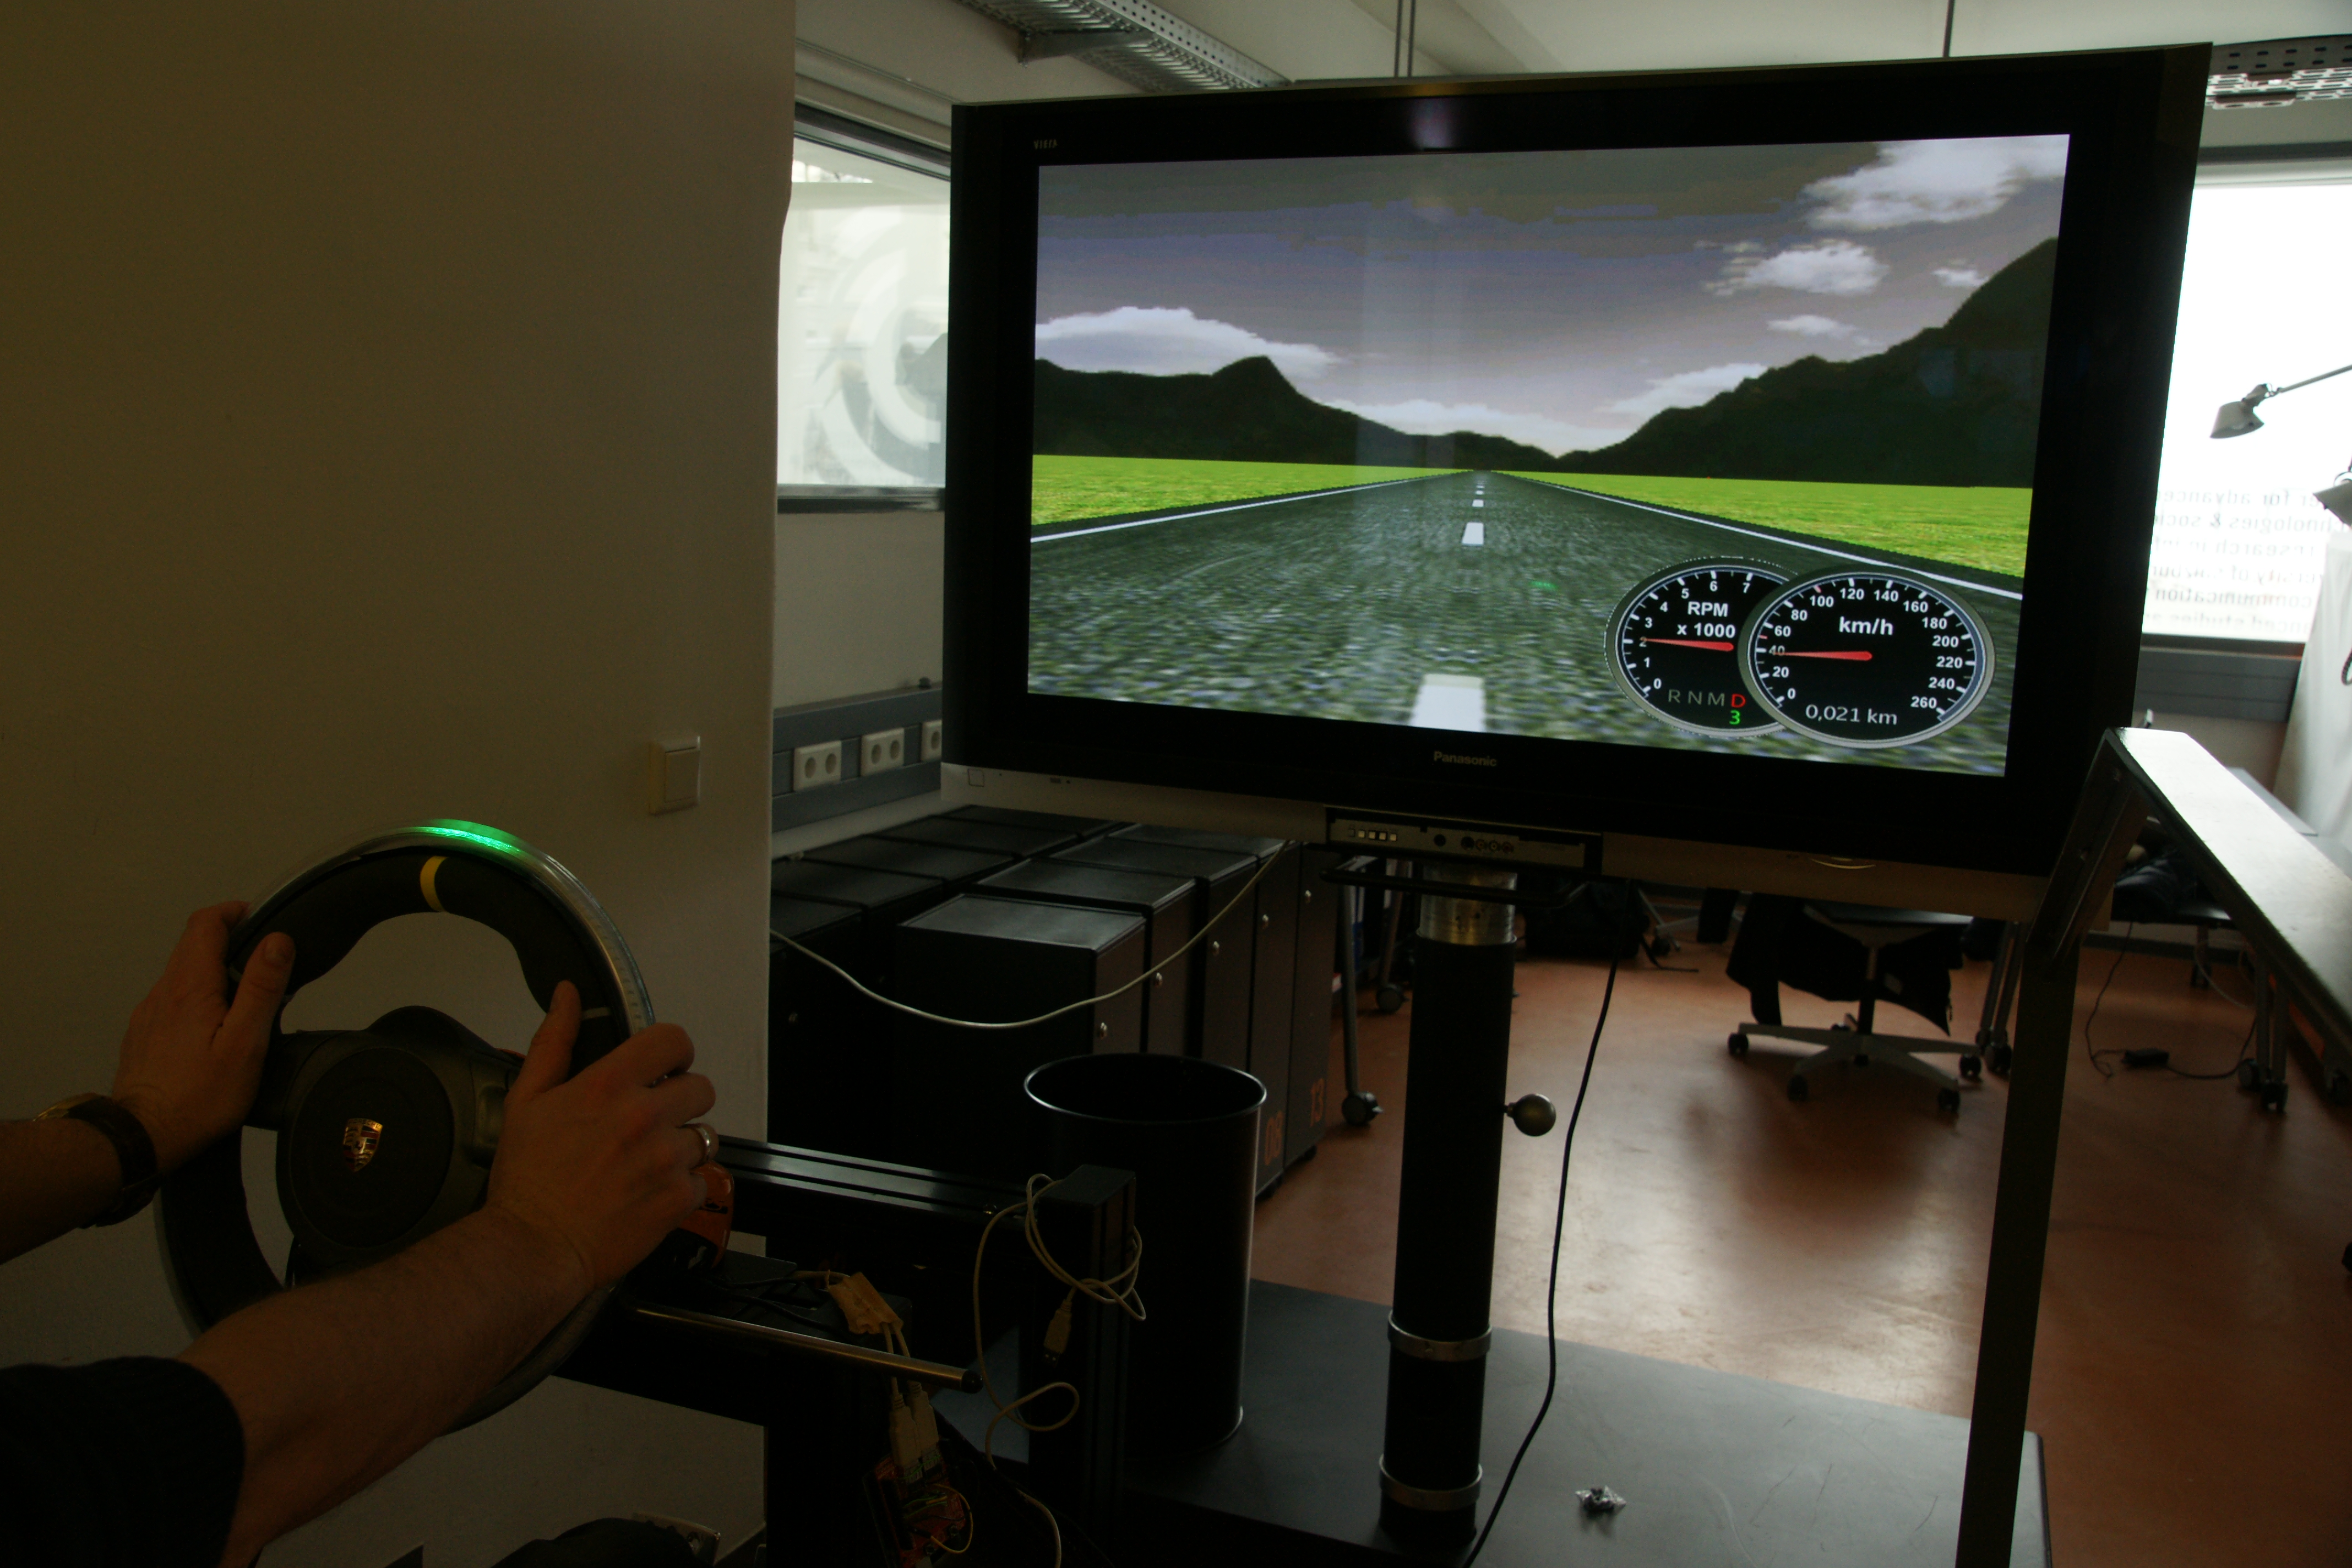
\includegraphics[width=12cm]{abb.jpg}
	\caption{Fahrsimulator Testumgebung mit LED-Lenkrad}
	\label{abb1}
\end{figure}
\end{center}
